\documentclass[journal]{vgtc}                % final (journal style)
%\documentclass[review,journal]{vgtc}         % review (journal style)
%\documentclass[widereview]{vgtc}             % wide-spaced review
%\documentclass[preprint,journal]{vgtc}       % preprint (journal style)

%% Uncomment one of the lines above depending on where your paper is
%% in the conference process. ``review'' and ``widereview'' are for review
%% submission, ``preprint'' is for pre-publication, and the final version
%% doesn't use a specific qualifier.

%% Please use one of the ``review'' options in combination with the
%% assigned online id (see below) ONLY if your paper uses a double blind
%% review process. Some conferences, like IEEE Vis and InfoVis, have NOT
%% in the past.

%% Please note that the use of figures other than the optional teaser is not permitted on the first page
%% of the journal version.  Figures should begin on the second page and be
%% in CMYK or Grey scale format, otherwise, colour shifting may occur
%% during the printing process.  Papers submitted with figures other than the optional teaser on the
%% first page will be refused. Also, the teaser figure should only have the
%% width of the abstract as the template enforces it.

%% These few lines make a distinction between latex and pdflatex calls and they
%% bring in essential packages for graphics and font handling.
%% Note that due to the \DeclareGraphicsExtensions{} call it is no longer necessary
%% to provide the the path and extension of a graphics file:
%% 
\includegraphics{diamondrule} is completely sufficient.
%%
\ifpdf%                                % if we use pdflatex
  \pdfoutput=1\relax                   % create PDFs from pdfLaTeX
  \pdfcompresslevel=9                  % PDF Compression
  \pdfoptionpdfminorversion=7          % create PDF 1.7
  \ExecuteOptions{pdftex}
  \usepackage{graphicx}                % allow us to embed graphics files
  \DeclareGraphicsExtensions{.pdf,.png,.jpg,.jpeg} % for pdflatex we expect .pdf, .png, or .jpg files
\else%                                 % else we use pure latex
  \ExecuteOptions{dvips}
  \usepackage{graphicx}                % allow us to embed graphics files
  \DeclareGraphicsExtensions{.eps}     % for pure latex we expect eps files
\fi%

%% it is recomended to use ``\autoref{sec:bla}'' instead of ``Fig.~\ref{sec:bla}''
\graphicspath{{figures/}{pictures/}{images/}{./}} % where to search for the images

\usepackage{microtype}                 % use micro-typography (slightly more compact, better to read)
\PassOptionsToPackage{warn}{textcomp}  % to address font issues with \textrightarrow
\usepackage{textcomp}                  % use better special symbols
\usepackage{mathptmx}                  % use matching math font
\usepackage{times}                     % we use Times as the main font
\renewcommand*\ttdefault{txtt}         % a nicer typewriter font
\usepackage{cite}                      % needed to automatically sort the references
%\usepackage{tabu}                      % only used for the table example
%\usepackage{booktabs}                  % only used for the table example
%% We encourage the use of mathptmx for consistent usage of times font
%% throughout the proceedings. However, if you encounter conflicts
%% with other math-related packages, you may want to disable it.

%% In preprint mode you may define your own headline.
%\preprinttext{To appear in IEEE Transactions on Visualization and Computer Graphics.}

%% If you are submitting a paper to a conference for review with a double
%% blind reviewing process, please replace the value ``0'' below with your
%% OnlineID. Otherwise, you may safely leave it at ``0''.
\onlineid{0}

%% declare the category of your paper, only shown in review mode
\vgtccategory{Research}
%% please declare the paper type of your paper to help reviewers, only shown in review mode
%% choices:
%% * algorithm/technique
%% * application/design study
%% * evaluation
%% * system
%% * theory/model
\vgtcpapertype{evaluation}

%% Paper title.
\title{Visualization of Malware across Business Sectors}

%% This is how authors are specified in the journal style

%% indicate IEEE Member or Student Member in form indicated below
\author{Emily Longman, Will Sims, and Taylor Kirkpatrick}

%other entries to be set up for journal
\shortauthortitle{Biv \MakeLowercase{\textit{et al.}}: Visualization of malware across business sectors}
%\shortauthortitle{Firstauthor \MakeLowercase{\textit{et al.}}: Paper Title}

%% Abstract section.
%%\abstract{ } % end of abstract

%% Keywords that describe your work. Will show as 'Index Terms' in journal
%% please capitalize first letter and insert punctuation after last keyword
\keywords{Security, malware}

%% ACM Computing Classification System (CCS). 
%% See <http://www.acm.org/class/1998/> for details.
%% The ``\CCScat'' command takes four arguments.

\CCScatlist{ % not used in journal version
 \CCScat{K.6.1}{Management of Computing and Information Systems}%
{Project and People Management}{Life Cycle};
 \CCScat{K.7.m}{The Computing Profession}{Miscellaneous}{Ethics}
}

%% Uncomment below to include a teaser figure.

%% Uncomment below to disable the manuscript note
%\renewcommand{\manuscriptnotetxt}{}

%% Copyright space is enabled by default as required by guidelines.
%% It is disabled by the 'review' option or via the following command:
% \nocopyrightspace

\vgtcinsertpkg

%%%%%%%%%%%%%%%%%%%%%%%%%%%%%%%%%%%%%%%%%%%%%%%%%%%%%%%%%%%%%%%%
%%%%%%%%%%%%%%%%%%%%%% START OF THE PAPER %%%%%%%%%%%%%%%%%%%%%%
%%%%%%%%%%%%%%%%%%%%%%%%%%%%%%%%%%%%%%%%%%%%%%%%%%%%%%%%%%%%%%%%%

\begin{document}

%% The ``\maketitle'' command must be the first command after the
%% ``\begin{document}'' command. It prepares and prints the title block.

%% the only exception to this rule is the \firstsection command
%%\firstsection{Introduction}

\maketitle

\section*{Introduction} %for journal use above \firstsection{..} instead
Cybersecurity is a serious concern, or at least should be, for almost every industry.
In the modern world relies heavily on computers of all forms, for basic tasks like checking the weather to heavy industrial computation.
The data stored and processed by these systems can be very valuable and targeted for theft.
Because of this there has been an ever-growing list of malware used to break into computer systems and gain whatever the attacker was looking for.
Today, with nearly 40 years of enterprise computer usage, there is a lot of data available on the exploits, but it can be very technical and hard to sift through. 
With information visualization we can do a better job on analyzing these trends, which allows the creation of better defenses against future attacks.

\section{Visualization Tasks}
The question we are trying to answer is what industries are most vulnerable to cyber attacks and what types of attacks are most prevalent. 
This problem is important because it provides a way for cybersecurity companies to see which industries are most in need of their services. 
It also allows industries that are most affected by cyber attacks to see which types of threats they are most vulnerable to.

\section{Data Sources}
There are plenty of security companies that disclose information about cyber attacks. 
Popular cyber security companies such as Symantec, McAfee, Malwarebytes publish monthly and yearly threat reports about different kinds of attacks. 
Symantec organizes the monthly threat report into five different categories: Malware, Web Attacks, Spam, Phishing, Mobile, and Social Media. 
They also give information about the number of threats per industry. \cite{SMR}
Malwarebytes publishes a state of malware report every year which contains information on the most common types of attacks with a focus on ransomware trends in particular. 
They give trends of different threats over the last three years, which provides a more thorough data set. \cite{MWB}
In the McAfee report, the volume of malicious samples cataloged per quarter ebbs and flows quarterly and annually. 
This data showed a decline during the past three quarters which mirrored the trend we observed at the start of 2015. 
A pattern of two to three quarters of growth followed by three quarters of decline has been consistent since 2013. \cite{QT17}

\section{Implementation}
We will implement the ER diagram by putting the data from Symantec into a mySQL database that is hosted by OSU using PHP.
We will have two tables, one that contains industries and the total number of attacks, along with threat ID’s that correspond to a type of threat, the number of attacks, and the date associated with the report. 
We can compare this data by looking at different sectors and how they vary by the attacks that are most common.

\section{ER Diagram}
The diagram for this project can be seen in Figure 1.
\begin{figure}[tb]
 \centering % avoid the use of \begin{center}...\end{center} and use \centering instead (more compact)
 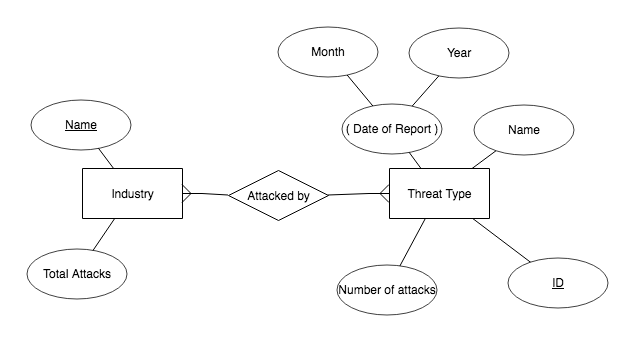
\includegraphics[width=\columnwidth]{erdigram}
 \caption{Layout of how different sources are related}
 \label{fig:sample}
\end{figure}

\section{Design Ideas}
\begin{figure}[tb]
 \centering % avoid the use of \begin{center}...\end{center} and use \centering instead (more compact)
 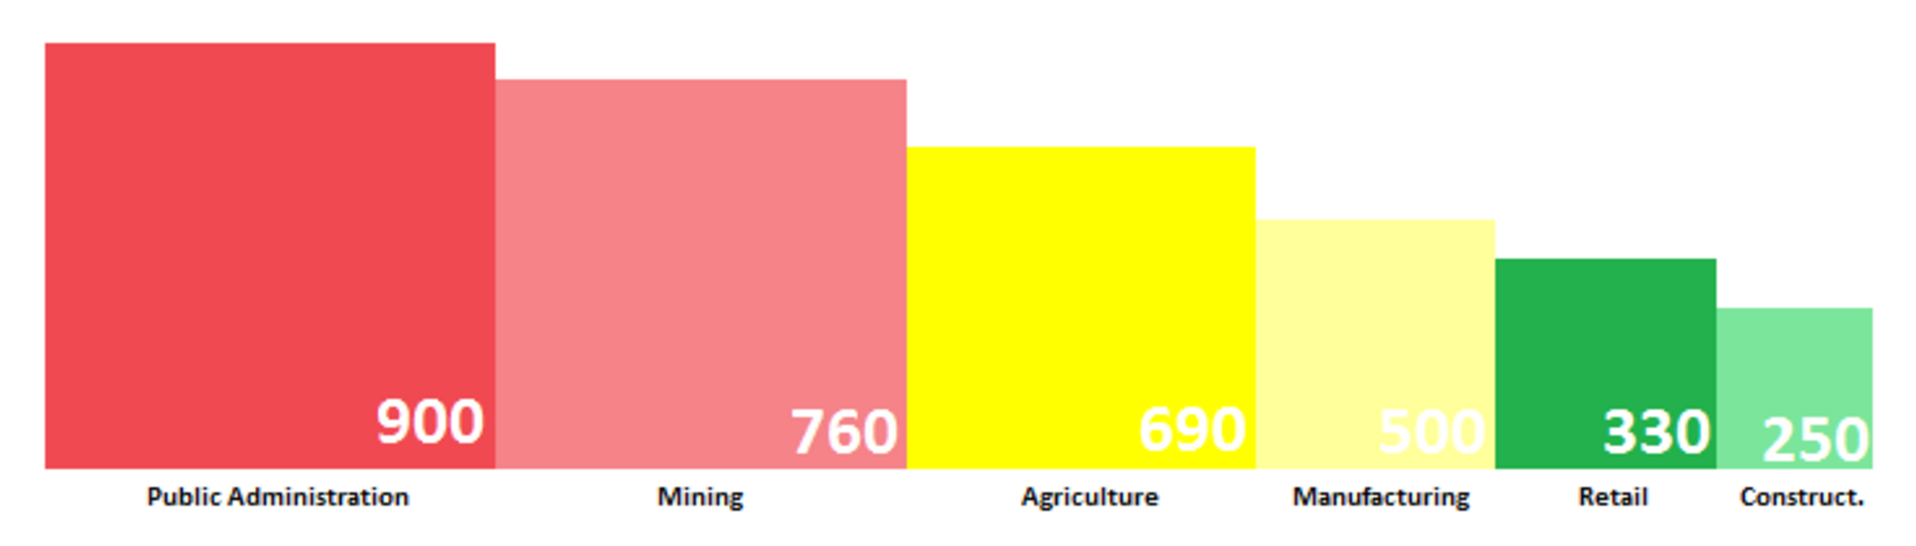
\includegraphics[width=\columnwidth]{Design1}
 \caption{Representation of attacks within different industries, utilizing color and size to represent the data visually}
 \label{fig:sample}
\end{figure}

This is the main part of the design, which can be seen in Figure 2. 
Each square represents an industry, labeled below it. 
The squares get larger and shift from green to yellow to red the more prevalent cyber attacks are in an industry. 
At a glance it is easy to tell which industry has the biggest problem with cyber attacks. 
Each box is labeled below, and inside the box is the total number of attacks per month (this is not real data). 
Something we put a lot of thought into while designing is the possibility of colorblind users, as they are quite common. 
In this part of the design, and in the rest, it should be noted that the design does not rely on color, and has an alternative way of conveying this information.

When hovering over any box with one’s mouse, say, the Agriculture box:
\begin{figure}[tb]
 \centering % avoid the use of \begin{center}...\end{center} and use \centering instead (more compact)
 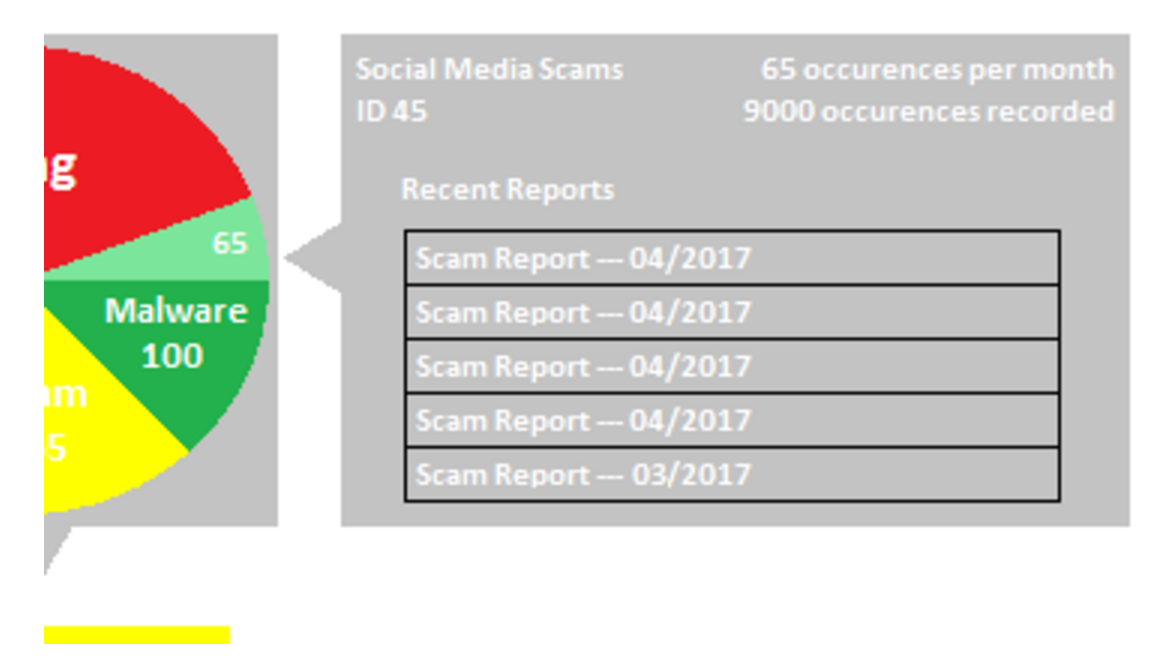
\includegraphics[width=\columnwidth]{Design2}
 \caption{Provides a breakdown of the prevalence of specific attack types within an industry}
 \label{fig:sample}
\end{figure}
You can see in Figure 3 that a pie chart has appeared above the square, with slices colored and sized based on cyber attack type. 
This shows the user a breakdown of not only what industry is subjected to attacks, but the distribution of attacks as well.
You might note the small size of the light green slice, and how there is only a number, not a label inside it. 
The is because the name cannot fit in the slice. 
The last part of the design can be seen by hovering over a slice to learn more about it.

For example, hovering over the small green slice: 
\begin{figure}[tb]
 \centering % avoid the use of \begin{center}...\end{center} and use \centering instead (more compact)
 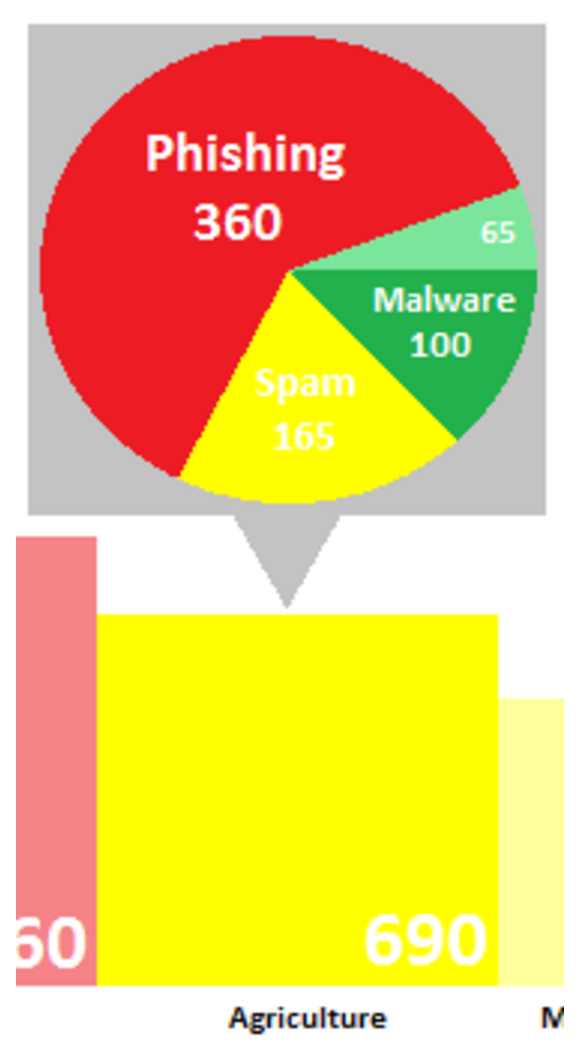
\includegraphics[width=\columnwidth]{Design3}
 \caption{A further breakdown, providing source details for each attack type}
 \label{fig:sample}
\end{figure}
This tab in figure 4 shows the detailed information we have about the attack, such as its name, the id we assign it, the occurrences per month (displayed on the slice) the total occurrences, and recent reports of the attack. 
This is a bit of a wall of text, but there isn’t much more we can do there, as this is detailed information that does not translate as well into a fancy graphic. 
This tab always opens to the right, to avoid running into taller industry squares.

\section{Conclusion}
This topic has a wide variety of data sources which can be combined and compared in interesting ways to draw a variety of conclusions.
With database manipulations and interesting front-end visualization this raw data can be made into something very interesting.
The better the visualization, the better users can understand the information and gain valuable security knowledge.


%\bibliographystyle{abbrv}
\bibliographystyle{abbrv-doi}
%\bibliographystyle{abbrv-doi-narrow}
%\bibliographystyle{abbrv-doi-hyperref}
%\bibliographystyle{abbrv-doi-hyperref-narrow}

\bibliography{secure_viz}
\end{document}

